%
% LaTeX Problem Set Template 
%

%%%%%%%%PACKAGES%%%%%%%%%%%%%%%%%%%%%%%%%%%%%%%%%%%%%%%%%%%%%%%%
\documentclass{article}
\usepackage{amsmath}
\usepackage{amssymb}
\usepackage{amsthm}
\usepackage{amssymb}
\usepackage{mathdots}
\usepackage{mathtools}
\usepackage[pdftex]{graphicx}
\usepackage{fancyhdr}
\usepackage[margin=1in]{geometry}
\usepackage{multicol}
\usepackage{bm}
\usepackage{listings}
\PassOptionsToPackage{usenames,dvipsnames}{color}  %% Allow color names
\usepackage{pdfpages}
\usepackage{algpseudocode}
\usepackage{tikz}
\usepackage{enumitem}
\usepackage[T1]{fontenc}
\usepackage{inconsolata}
\usepackage{framed}
\usepackage{wasysym}
\usepackage[thinlines]{easytable}
\usepackage{hyperref}
\usepackage{wrapfig}
\usepackage[makeroom]{cancel}
\usepackage{tikz, wasysym}
\usetikzlibrary{automata,positioning, arrows.meta, calc}
\hypersetup{
    colorlinks=true,
    linkcolor=blue,
    filecolor=magenta,
    urlcolor=blue,
}
\delimiterfactor = 1200
%%%%%%%%%%%%%%%%%%%%%%%%%%%%%%%%%%%%%%%%%%%%%%%%%%%%%%%%
\title{CMSI 3802: Languages \& Automata \\ Homework 4}
\author{[Ryan Ramsdell (980388983)]}
\date{\today}
\makeatletter
\let\runauthor\@author
\makeatother

\lhead{\runauthor}
\chead{HW 4}
\rhead{\today}
\lfoot{}
\rfoot{\thepage}
%%%%%%%%%%%%%%%%%%%%%%%%%%%%%%%%%%%%%%%%%%%%%%%%%%%%%%%%

% start MZ
\let\oldemptyset\emptyset
\renewcommand{\emptyset}{\text{\O}}
\renewcommand{\labelitemii}{$\bullet$}
\renewcommand\qedsymbol{$\blacksquare$}
\newenvironment{prf}{{\bfseries Proof.}}{\qedsymbol}
\renewcommand{\emph}[1]{\textit{\textbf{#1}}}
\newcommand{\annotate}[1]{\textit{\textcolor{blue}{#1}}}
\usepackage{mdframed}
\usepackage{float}

\makeatother
% end MZ

\definecolor{shadecolor}{gray}{0.95}

\renewcommand{\headrulewidth}{0.4pt}
\renewcommand{\footrulewidth}{0.4pt}

\setlength{\parindent}{0pt}

\pagestyle{fancy}

\renewcommand{\thefootnote}{\fnsymbol{footnote}}

\DeclarePairedDelimiter{\ceil}{\lceil}{\rceil}
%%%%%%%%%%%%%%%%Document Begins Here!%%%%%%%%%%%%%%%%%%%%%%%%
\begin{document}

\maketitle

\section*{Problem 1}
\begin{enumerate}[label=(\alph*)]
  \item Language Theory
    \begin{shaded}
      It deals with the expression of computation and information, analyzing how alphabets can compute functions.
    \end{shaded}
  \item Automata Theory
    \begin{shaded}
      It analyzes specific, formal models of computers, including things like the turing machine, pascal's adder, and more.
    \end{shaded}
  \item Computability Theory
    \begin{shaded}
      It is the discussion of whether or not every possible function can be computed, the answer being "no"; specificially, a function that knows if a given program will terminate.
    \end{shaded}
  \item Complexity Theory
    \begin{shaded}
      Complexity theory is similar to computability theory, but specifically with reguard to how long a function will take to compute.
    \end{shaded}
\end{enumerate}

\section*{Problem 2}
\begin{enumerate}[label=(\alph*)]
  \item $L_1 \cup L_2$
    \begin{shaded}
      $\{1, 011, 10, 1\}$
    \end{shaded}
  \item $L_1 \cap L_2$
    \begin{shaded}
      $\{10\}$
    \end{shaded}
  \item $L_1 L_2$
    \begin{shaded}
      $\{010, 01, 01110, 0111, 1010, 101\}$
    \end{shaded}
  \item $L_2^*$
    \begin{shaded}
      $\{\epsilon, 10, 1, 11, 101, 110, 1010, ...\}$
    \end{shaded}
\end{enumerate}


\section*{Problem 3}
\begin{enumerate}[label=(\alph*)]
  \item The empty language
    \begin{shaded}
      $S \rightarrow (no rules)$
    \end{shaded}

  \item $\{ 0^i1^j2^k \mid i=j \lor j=k \}$
    \begin{shaded}
      \begin{align*}
        S &\rightarrow 0S1 \,|\, A \\
        A &\rightarrow 1A2 \,|\, B                &(\text{for } i=j) \\
        B &\rightarrow 0B \,|\, 2B \,|\, \epsilon &(\text{for } j=k)
      \end{align*}
    \end{shaded}

  \item $\{ w \in \{0,1\}^* \mid w \textrm{ does not contain the substring 000} \}$
    \begin{shaded}
      \begin{align*}
        S &\rightarrow 0S \,|\, 01S \,|\, 001S \,|\, 1S \,|\, \epsilon
      \end{align*}
    \end{shaded}

  \item $\{ w \in \{a,b\}^* \mid w \textrm{ has twice as many $a$'s as $b$'s} \}$
    \begin{shaded}
      \begin{align*}
        S &\rightarrow aSaSb \,|\, ab \,|\, \epsilon
      \end{align*}
    \end{shaded}

  \item $\{ a^nb^na^nb^n \mid n \geq 0 \}$
    \begin{shaded}
      \begin{align*}
        S &\rightarrow aSb \,|\, T \\
        T &\rightarrow aTb \,|\, \epsilon
      \end{align*}  
    \end{shaded}
\end{enumerate}

\section*{Problem 4}
\begin{shaded}
  $$
  \begin{aligned}
      V &= \{n, f, e, d, D, E, E', F\} \\
      \Sigma &= \{\text{"0"}, \text{"1"}, \text{"2"}, \text{"3"}, \text{"4"}, \text{"5"}, \text{"6"}, \text{"7"}, \text{"8"}, \text{"9"}, \text{"."}, \text{"E"}, \text{"e"}, \text{"+"}, \text{"–"}\} \\
      R &= \left\{ 
      \begin{aligned}
        n  &\rightarrow dD \,|\, dDF \,|\, dDE \,|\, dDFE \\
        D  &\rightarrow dD \,|\, d \\
        F  &\rightarrow \text{"."}dD \\
        E  &\rightarrow \text{"E"}E' \,|\, \text{"e"}E' \\
        E' &\rightarrow dD \,|\, \text{"+"}dD \,|\, \text{"-"}dD \\
        d  &\rightarrow \text{"0".."9"} \\
      \end{aligned}
      \right\} \\
      S &= n
  \end{aligned}
  $$
\end{shaded}

\section*{Problem 5}
Give Turing Machines that recognize the following languages. If any of the languages below are Type-3, you may (and are encouraged to) give a FA in lieu of a TM recognizer, if the FA is simpler.
\begin{enumerate}[label=(\alph*)]
  \item $\{w \in \{a,b\}* \mid w \textrm{ ends with } abb\}$
    \begin{shaded}
      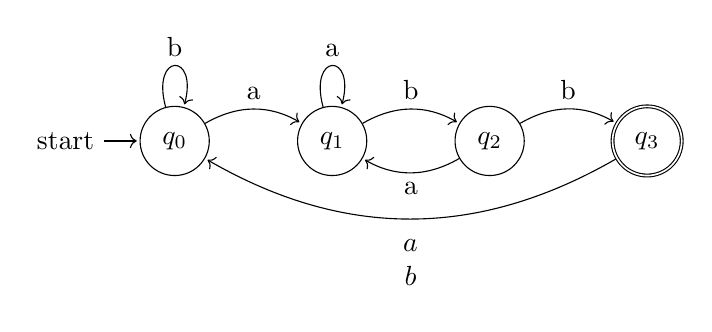
\begin{tikzpicture}[shorten >=1pt, node distance=2cm, on grid, auto]
        \node[state, initial]   (0)              {$q_0$};
        \node[state]            (1) [right=of 0] {$q_1$};
        \node[state]            (2) [right=of 1] {$q_2$};
        \node[state, accepting] (3) [right=of 2] {$q_3$};

        \path[->]
          (0) edge [loop above] node {b} (1)
          (0) edge [bend left]  node {a} (1)

          (1) edge [bend left]  node {b} (2)
          (1) edge [loop above] node {a} (1)

          (2) edge [bend left]  node {b} (3)
          (2) edge [bend left]  node {a} (1)
          (3) edge [bend left]  node {$\begin{matrix}a\\b\end{matrix}$} (0);
      \end{tikzpicture}
    \end{shaded}

  \item $\{ w \in \{a,b\}^* \mid \#_a(w) = \#_b(w) \}$ (same number of $a$'s and $b$'s)
    \begin{shaded}
      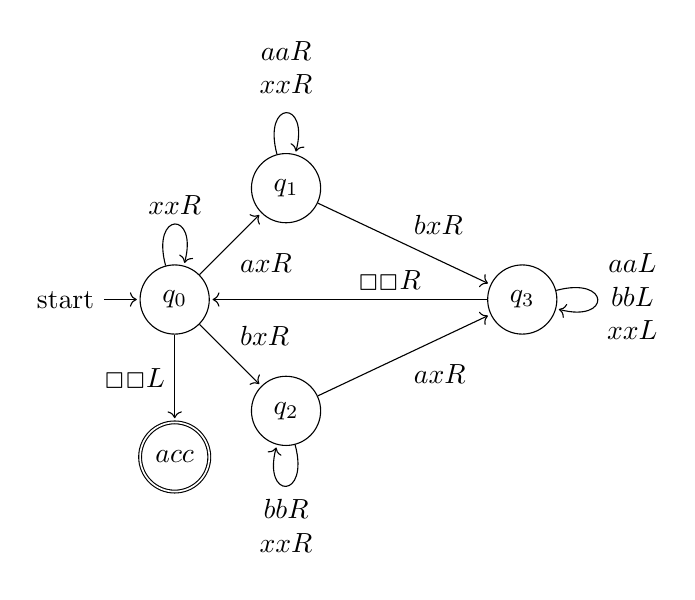
\begin{tikzpicture}[shorten >=1pt, node distance=2cm, on grid, auto]
        \node[state, initial]                      (0)   {$q_0$};
        \node[state, accepting] [below=of 0]       (acc) {$acc$};

        \node[state]            [above right=of 0] (1)   {$q_1$};
        \node[state]            [below right=of 0] (2)   {$q_2$};

        \node[state] (3) at ($(1)!0.5!(2) + (3cm, 0)$)   {$q_3$};

        \path[->]
          (0) edge [loop above] node {$xxR$} (0)
          (0) edge              node [left] {$\Box\Box L$} (acc)

          (0) edge              node [below right] {$axR$} (1)
          (1) edge              node [above right] {$bxR$} (3)
          (1) edge [loop above] node [above] {$\begin{matrix}aaR\\xxR\end{matrix}$} (1)

          (0) edge              node [above right] {$bxR$} (2)
          (2) edge              node [below right] {$axR$} (3)
          (2) edge [loop below] node [below] {$\begin{matrix}bbR\\xxR\end{matrix}$} (2)

          (3) edge [loop right] node [right] {$\begin{matrix}aaL\\bbL\\xxL\\\end{matrix}$} (3)
          (3) edge              node [above right] {$\Box\Box R$} (0);

      \end{tikzpicture}
    \end{shaded}

  \item $\{w \in \{a,b\}* \mid w \textrm{ alternates } a\textrm{'s and } b\textrm{'s} \}$
    \begin{shaded}
      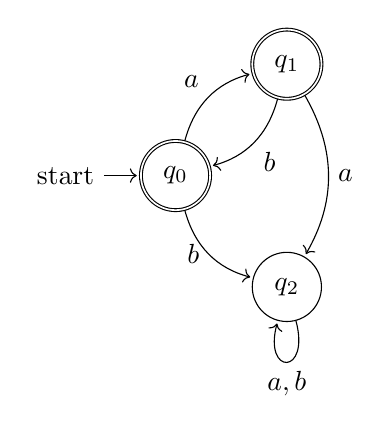
\begin{tikzpicture}[shorten >=1pt, node distance=2cm, on grid, auto]
        \node[state, initial, accepting] (0) {$q_0$};
        \node[state, accepting] (1) [above right=of 0] {$q_1$};
        \node[state] (2) [below right=of 0] {$q_2$};
     
        \path[->]
          (0) edge [bend left]  node        {$a$}    (1)
          (0) edge [bend right] node [left] {$b$}    (2)
               
          (1) edge [bend left]  node        {$b$}    (0)
          (1) edge [bend left]  node        {$a$}    (2)

          (2) edge [loop below] node        {$a, b$} (2);
     \end{tikzpicture}
    \end{shaded}

  \item $\{ a^nb^na^nb^n \mid n \geq 0 \}$
    \begin{shaded}
      Note: Apologies for the messy diagram, I spent like 45 minutes on this one trying to get \LaTeX to format it nicely, and I decided to just take the L.\\
      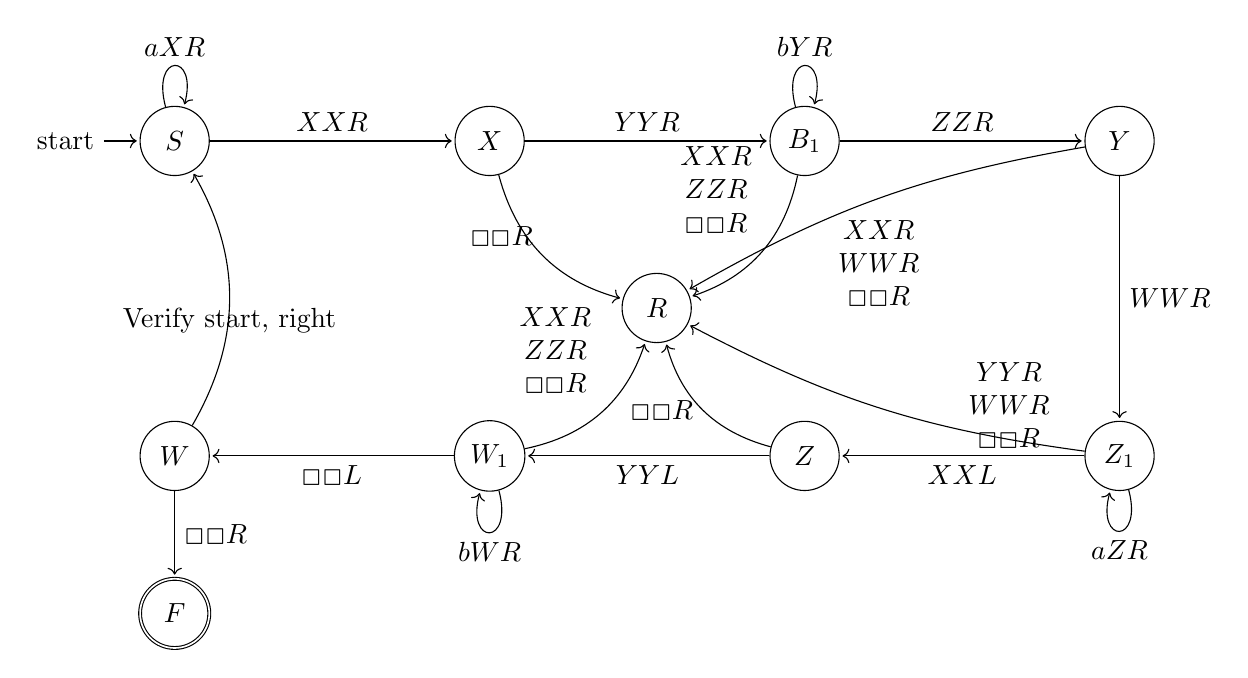
\begin{tikzpicture}[shorten >=1pt, node distance=4cm, on grid, auto]
        \node[state,initial]    (S)                {$S$};
        \node[state]            (X)  [right of=S] {$X$};
        \node[state]            (B1) [right of=X]{$B_1$};
        \node[state]            (Y)  [right of=B1]{$Y$};
        \node[state]            (Z1) [below of=Y]{$Z_1$};
        \node[state]            (Z)  [left of=Z1] {$Z$};
        \node[state]            (W)  [below of=S] {$W$};
        \node[state]            (W1) [right of=W] {$W_1$};
        \node[state,accepting]  (F)  [below=2cm of W] {$F$};
        \node[state]            (R)  [below right=3cm of X] {$R$};
        
        \path[->]
          (S)     edge node {$XXR$} (X)
                  edge[loop above] node {$aXR$} (S)
          (X) edge node {$YYR$} (B1)
          (B1) edge[loop above] node {$bYR$} (B1)
                  edge node {$ZZR$} (Y)
          (Y) edge node {$WWR$} (Z1)
          (Z1) edge[loop below] node {$aZR$} (Z1)
                  edge node {$XXL$} (Z)
          (Z) edge node {$YYL$} (W1)
          (W1) edge[loop below] node {$bWR$} (W1)
                  edge node {$\Box\Box L$} (W)
          (W) edge node {$\Box\Box R$} (F)
                  edge[bend right] node[below] {Verify start, right} (S)
          (X) edge[bend right] node[above left]{$\Box\Box R$} (R)
          (B1) edge[bend left] node[above left]{$\begin{matrix}XXR\\ZZR\\ \Box\Box R\end{matrix}$} (R)
          (Y) edge[bend right=10] node[below=0.1cm]{$\begin{matrix}XXR\\WWR\\ \Box\Box R\end{matrix}$} (R)
          (Z1) edge[bend left=10] node[right=1cm]{$\begin{matrix}YYR\\WWR\\ \Box\Box R\end{matrix}$} (R)
          (Z) edge[bend left] node[left]{$\Box\Box R$} (R)
          (W1) edge[bend right] node[above left]{$\begin{matrix}XXR\\ZZR\\ \Box\Box R\end{matrix}$} (R);
      \end{tikzpicture}
    \end{shaded}
\end{enumerate}

\section*{Problem 6}
Give Turing Machines that compute the following functions, where the input and output are binary numerals.
\begin{enumerate}[label=(\alph*)]
  \item $\lambda n. 2n + 2$
    \begin{shaded}
      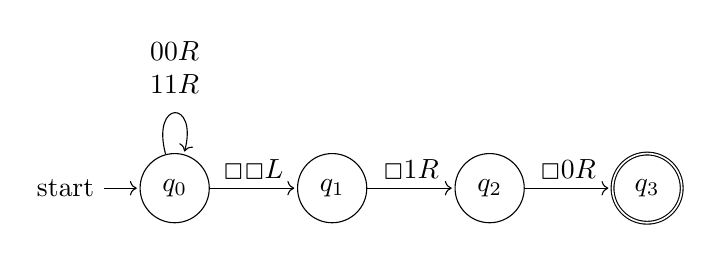
\begin{tikzpicture}[shorten >=1pt, node distance=2cm, on grid, auto]
        \node[state, initial]   (0)              {$q_0$};
        \node[state]            (1) [right=of 0] {$q_1$};
        \node[state]            (2) [right=of 1] {$q_2$};
        \node[state, accepting] (3) [right=of 2] {$q_3$};

        \path[->]
          (0) edge [loop above] node {$\begin{matrix}00R\\11R\end{matrix}$} (0)
          (0) edge              node {$\Box\Box L$} (1)
          (1) edge              node {$\Box 1R$}    (2)
          (2) edge              node {$\Box 0R$}    (3);
      \end{tikzpicture}
    \end{shaded}

  \item one's complement
    \begin{shaded}
      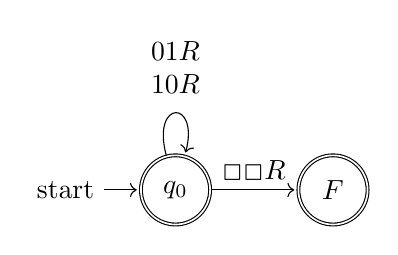
\begin{tikzpicture}[shorten >=1pt, node distance=2cm, on grid, auto]
        \node[state, initial, accepting]   (0)              {$q_0$};
        \node[state, accepting]            (F) [right=of 0] {$F$};

        \path[->]
          (0) edge [loop above] node {$\begin{matrix}01R\\10R\end{matrix}$} (0)
          (0) edge              node {$\Box\Box R$} (F);
      \end{tikzpicture}
    \end{shaded}

  \item The function described in Python as \verb|lambda n: str(n)[1:-1]|
    \begin{shaded}
      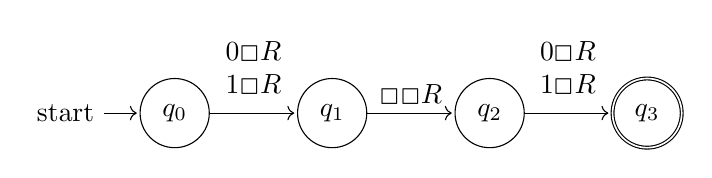
\begin{tikzpicture}[shorten >=1pt,node distance=2cm,on grid,auto] 
        \node[state,initial] (q_0)   {$q_0$}; 
        \node[state] (q_1) [right=of q_0] {$q_1$}; 
        \node[state] (q_2) [right=of q_1] {$q_2$}; 
        \node[state,accepting](q_3) [right=of q_2] {$q_3$};
         \path[->] 
         (q_0) edge  node {$\begin{matrix}0\Box R\\1 \Box R\end{matrix}$} (q_1)
         (q_1) edge  node {$\Box \Box R$} (q_2)
         (q_2) edge  node {$\begin{matrix}0\Box R\\1 \Box R\end{matrix}$} (q_3);
     \end{tikzpicture}
    \end{shaded}

  \item Maximum bit-string length of two numerals, after leading zeros are removed, where the input is the two numerals separated by a single blank
    \begin{shaded}
      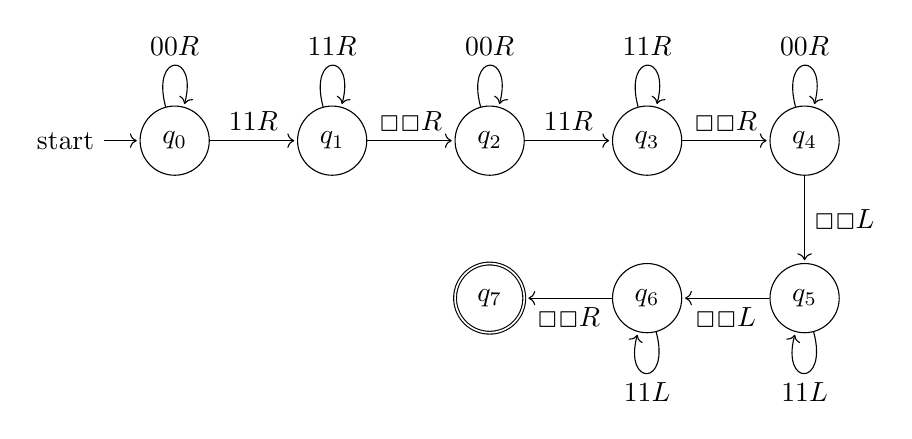
\begin{tikzpicture}[shorten >=1pt,node distance=2cm,on grid,auto] 
        \node[state,initial] (q_0)   {$q_0$}; 
        \node[state] (q_1) [right=of q_0] {$q_1$}; 
        \node[state] (q_2) [right=of q_1] {$q_2$}; 
        \node[state] (q_3) [right=of q_2] {$q_3$};
        \node[state] (q_4) [right=of q_3] {$q_4$};
        \node[state] (q_5) [below=of q_4] {$q_5$};
        \node[state] (q_6) [left=of q_5] {$q_6$};
        \node[state,accepting](q_7) [left=of q_6] {$q_7$};
         \path[->] 
         (q_0) edge [loop above] node {$00R$} ()
               edge node {$11R$} (q_1)
         (q_1) edge [loop above] node {$11R$} ()
               edge node {$\Box\Box R$} (q_2)
         (q_2) edge [loop above] node {$00R$} ()
               edge node {$11R$} (q_3)
         (q_3) edge [loop above] node {$11R$} ()
               edge node {$\Box\Box R$} (q_4)
         (q_4) edge [loop above] node {$00R$} ()
               edge node {$\Box\Box L$} (q_5)
         (q_5) edge [loop below] node {$11L$} ()
               edge node {$\Box\Box L$} (q_6)
         (q_6) edge [loop below] node {$11L$} ()
               edge node {$\Box\Box R$} (q_7);
     \end{tikzpicture}
    \end{shaded}
\end{enumerate}

\section*{Problem 6}
For the JavaScript/Python expression \verb|5 * 3 - 1 ** 3|,
\begin{enumerate}[label=(\alph*)]
  \item Show a 3AC machine program to evaluate this expression, leaving the result in $r_0$
    \begin{shaded}
      \begin{verbatim}
        COPY 5, r1
        COPY 3, r2
        MUL r1, r2, r3

        COPY 1, r4
        COPY 3, r5
        POW r4, r5, r6

        SUB r3, r6, r0

        WRITE r0
        HALT
      \end{verbatim}
    \end{shaded}

  \item Show a Stack machine program to evaluate this expression, leaving the result on the top of the stack.
    \begin{shaded}
      \begin{verbatim}
        PUSH 5
        PUSH 3
        MULT
        PUSH 1
        PUSH 3
        POW
        SUB
      \end{verbatim}
    \end{shaded}
\end{enumerate}

\section*{Problem 8}
Characterize each of the following languages as either (a) regular, (b) context-free but not regular, (c) recursive but not context-free, (d) recursively enumerable but not recursive, or (e) not even recursively enumerable.
\begin{enumerate}[label=(\alph*)]
  \item $\{ a^ib^jc^k \mid i > j > k \}$
    \begin{shaded}
      c: recursive but not context-free
    \end{shaded}

  \item $\{ a^ib^jc^k \mid i > j \wedge k \leq i-j \}$
    \begin{shaded}
      c: recursive but not context-free
    \end{shaded}

  \item $\{ \hat{M}w \mid M \textrm{ accepts } w\}$
    \begin{shaded}
      d: recursively enumerable but not recursive
    \end{shaded}

  \item $\{ G \mid G \textrm{ is context-free} \wedge L(G)=\varnothing \}$
    \begin{shaded}
      c: recursive but not context-free
    \end{shaded}

  \item $\{ a,b \}^*\{b\}^+$
    \begin{shaded}
      a: regular
    \end{shaded}

  \item $\{ \hat{M} \mid M \textrm{ does not halt }\}$
    \begin{shaded}
      e: not even recursively enumerable
    \end{shaded}

  \item $\{ w \mid w \textrm{ is a decimal numeral divisible by 7} \}$
    \begin{shaded}
      a: regular
    \end{shaded}

  \item $\{ www \mid w \textrm{ is a string over the Unicode alphabet} \}$
    \begin{shaded}
      c: recursive but not context-free
    \end{shaded}

\end{enumerate}

\end{document}